\section{Introduction}
Learning-based robot manipulation requires visual representations that describe not only what is currently visible, but also how the scene should change for a task to succeed. While recent advances in visual representation learning have enabled frozen visual features to support robotic perception and control, manipulation is inherently temporal, as effective control requires a policy to identify which object motion, contact event, or configuration change matters next. However, many generic representations either lack temporal knowledge or encode it only implicitly. Static features do not directly indicate how the scene is expected to evolve, forcing downstream controllers to infer task-relevant dynamics from limited demonstrations~\cite{hewage2020temporal,zakka2022xirl}. 

% \CO{As illustrated in Fig.~\ref{fig:teaser}, this static representation contrasts with TRAIL's explicit latent change signal. Learning this temporal structure without robot-specific pre-training data or dense manual supervision remains a central challenge~\cite{schmidt2024learning,ye2025latent}.}

\begin{figure}[t]
    \centering
    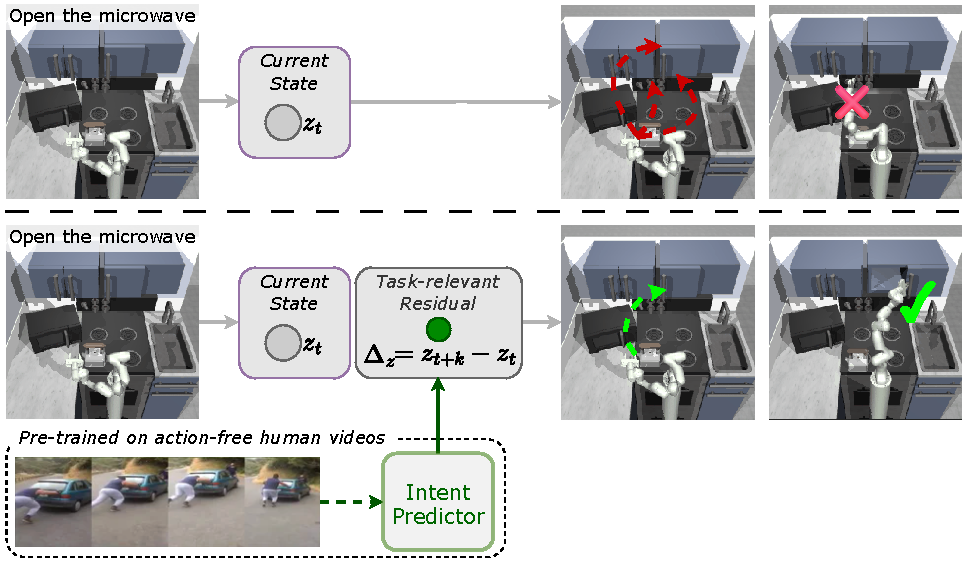
\includegraphics[width=\linewidth]{ieeeconf/figure/teaser_cropped.pdf}
    \caption{\textbf{Overview.}
        (Top) Frozen visual representations provide the policy with the current visual state, leaving the downstream controller to infer task-relevant changes.
        (Bottom) Our method uses the intent stream that provides task-relevant residual $\Delta_z$ as context for the closed-loop policy.}
    \label{fig:teaser}
\end{figure}



Predictive representation learning provides a natural way to model these temporal changes, while existing predictive pipelines do not directly employ a control-oriented change signal to the policy. Future prediction has long been used to learn dynamics useful for decision making~\cite{hafner2019dream,finn2017deep}. In vision-based representation learning, many methods train by reconstructing or predicting future visual content~\cite{he2022masked,gupta2023siamese,zhu2025lava,zeng2024learning,karamcheti2023language,kim2025token}. Such objectives can allocate capacity to visual details that are not decisive for manipulation. Moreover, the temporal component is often discarded or compressed after pre-training: predictive decoders may be removed before downstream learning~\cite{radosavovic2023real,xiao2022masked}, while objectives such as time-contrastive learning~\cite{nair2022r3m} leave temporal information only implicitly inside a static embedding. The fundamental technical problem is therefore not simply how to learn future prediction, but how to retain the task-relevant part of prediction as an explicit policy input.

We propose TRAIL (\textbf{T}ask-\textbf{R}elevant residuals as an \textbf{A}ction prior for robot man\textbf{I}pu\textbf{L}ation), a self-supervised framework that learns a task-relevant latent change from action-free human videos\footnote{For more results: \url{https://anonymous.4open.science/w/ICRA2027-E3D6/index.html}}. TRAIL defines current and future states in a frozen visual feature space and trains a shared future predictor with asymmetric visual access. The full-information stream uses the global visual token,
dense visual patch tokens, and grounded language context, while the intent stream uses only the global visual token and language context. 
Distilling the full-information prediction into the intent stream encourages the model to capture task-relevant future changes rather than generic background motion or passive scene changes. At deployment, we use the intent stream to predict the task-relevant future latent and compute its residual from the current state. We design the policy conditioned on both the current representation and this residual, providing an explicit task-relevant change signal for downstream control.

% At deployment, TRAIL strengthens prediction with residual-guided policy representation. The retained intent stream is executed at every control step, producing a task-relevant latent forecast in the same feature space as the current observation. TRAIL then computes the token-wise latent residual $\Delta_z$ between the forecast and the current state, and feeds both the current state and this residual to the downstream policy. This design differs from using an absolute future feature alone by providing the residual that indicates the tendency of future movement. In this way, the task burden placed on the action decoder is greatly alleviated, leading to more robust and effective adaptation to downstream robotic tasks.

% Our experiments evaluate whether this retained latent residual improves downstream control under fixed policy-learning protocols. On Franka Kitchen~\cite{franka_kitchen}, TRAIL achieves the highest average success rate among the compared frozen-representation and predictive baselines. On Meta-World MT10~\cite{yu2020meta}, TRAIL again obtains the strongest average result, with the clearest gains on tasks where object motion makes the next action depend on how the scene is changing. In real-robot tabletop manipulation, TRAIL improves average success over CLIPort~\cite{shridhar2022cliport}, MPI~\cite{zeng2024learning}, and LaVA-Man~\cite{zhu2025lava}, with strong results on held-out objects and contact-rich pushing tasks. 

Our contributions are summarized as follows:

\begin{itemize}
    \item We introduce an asymmetric predictive representation learning framework that captures task-relevant latent dynamics from action-free human videos.
    \item We propose to retain the trained predictor and explicitly feed the task-relevant latent change signal to downstream policies as part of their context.
\end{itemize}

Experiments on two simulated benchmarks, Franka Kitchen~\cite{franka_kitchen} and Meta-World MT10~\cite{yu2020meta}, and seven real-robot manipulation tasks demonstrate consistent improvements over existing visual and predictive representations.